\chapter{\IfLanguageName{dutch}{Automatisatie}{Automatisation}}%
\label{ch:automatisatie}

\section{Structuur van de Playbook}
\label{sec:playbookstructuur}

\subsection{Connectie met remote hosts}

\subsection{Gebruik van Jinja2 voor templating}

\subsection{Security}

\section{Werking van de Playbook}
\label{sec:playbookwerking}

\begin{figure}[H]
    \centering
    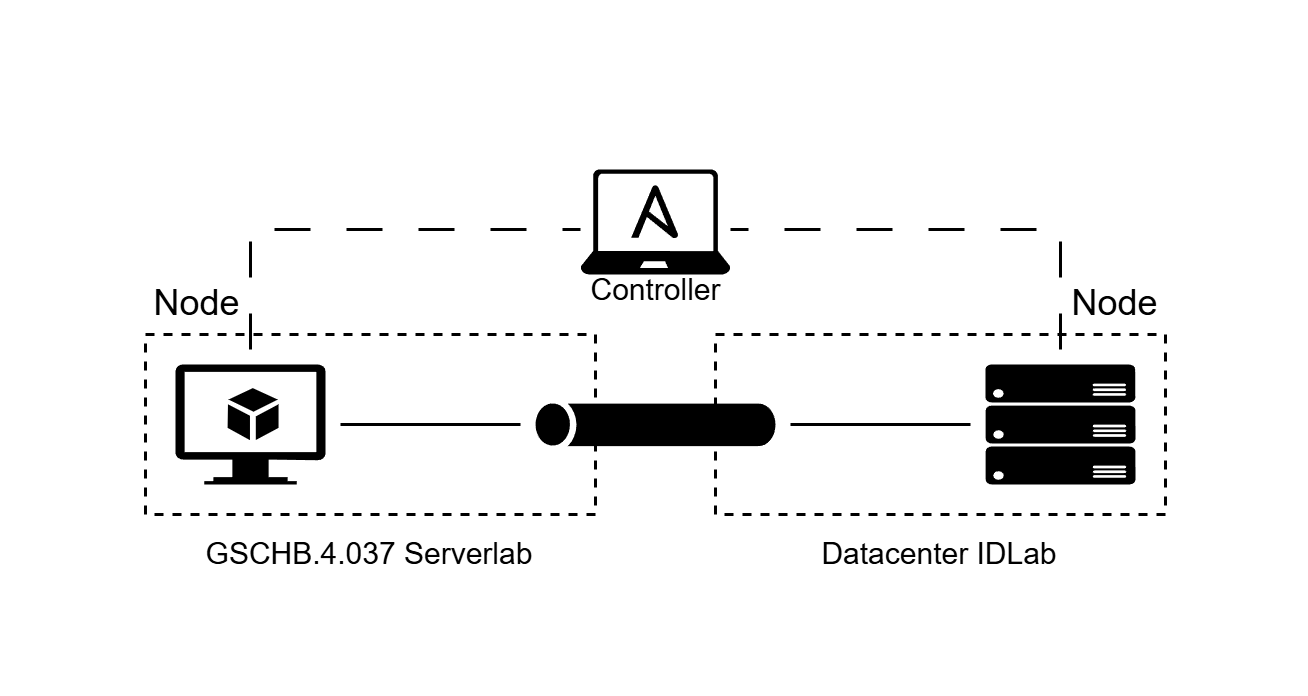
\includegraphics[width=1\textwidth]{ConnectieAnsible.png}
    \caption[Overzicht van hoe de connectie praktish in elkaar zit.]{\label{fig:ansibleconnectie}Overzicht van hoe de connectie praktish in elkaar zit.}
\end{figure}